\let\negmedspace\undefined
\let\negthickspace\undefined
\documentclass[journal]{IEEEtran}
\usepackage[a5paper, margin=10mm, onecolumn]{geometry}
%\usepackage{lmodern} 
\usepackage{tfrupee} 

\setlength{\headheight}{1cm} 
\setlength{\headsep}{0mm}     

\usepackage{gvv-book}
\usepackage{gvv}
\usepackage{cite}
\usepackage{amsmath,amssymb,amsfonts,amsthm}
\usepackage{algorithmic}
\usepackage{graphicx}
\usepackage{textcomp}
\usepackage{xcolor}
\usepackage{txfonts}
\usepackage{listings}
\usepackage{enumitem}
\usepackage{mathtools}
\usepackage{gensymb}
\usepackage{comment}
\usepackage[breaklinks=true]{hyperref}
\usepackage{tkz-euclide} 
\usepackage{listings}                                        
\def\inputGnumericTable{}                                 
\usepackage[latin1]{inputenc}                                
\usepackage{color}                                            
\usepackage{array}                                            
\usepackage{longtable}                                       
\usepackage{calc}                                             
\usepackage{multirow}                                         
\usepackage{hhline}                                           
\usepackage{ifthen}                                           
\usepackage{lscape}

\begin{document}

\bibliographystyle{IEEEtran}
\vspace{3cm}

\title{12.705}
\author{AI25BTECH11003 - Bhavesh Gaikwad}
{\let\newpage\relax\maketitle}

\renewcommand{\thefigure}{\theenumi}
\renewcommand{\thetable}{\theenumi}
\setlength{\intextsep}{10pt} 

\numberwithin{equation}{enumi}
\numberwithin{figure}{enumi}
\renewcommand{\thetable}{\theenumi}


\textbf{Question}: The minimum value of y for the equation $y = x^2 - 2x + 4$ is

\hfill{(MT 2021)}

\begin{itemize}
    \item[a)]3
    \item[b)]1
    \item[c)]4
    \item[d)]6
\end{itemize}

\bigskip

 \solution 
 \\
Given:
\begin{equation}
  Parabola: \;  x^2 - 2x - y + 4 =0
\end{equation}


Parameters of the Parabola:
\begin{equation}
    \vec{V} = \myvec{1 & 0 \\ 0 & 0}, \quad \vec{u} = \myvec{-1 \\ -1/2}, \quad f = 4
\end{equation}

Equation of Parabola:
\begin{equation}
\vec{X}^\top\myvec{1 & 0 \\ 0 & 0}\vec{X} + 2\myvec{-1 & -1/2}\vec{X} + 4 = 0    
\end{equation}

Let line $L$ be parallel to the x-axis and passes through $y_{min}$.\\
Let $\phi$ represent the minimum value of $y$.
\begin{equation}
    \therefore \; L: \, \vec{X} = k\myvec{ 1 \\ 0} + \myvec{0 \\ \phi}
\end{equation}

Parameters of Line $L$:
\begin{equation}
\vec{m}= \myvec{1 \\ 0}, \quad \vec{h} = \myvec{0 \\ \phi}    
\end{equation}

Intersection of $L$ with Parabola:
\begin{equation}
    \vec{x}_i = k_i\vec{m} + \vec{h}
\end{equation}

\begin{equation}
    k_i = \dfrac{1}{\vec{m}^\top\vec{V}\vec{m}}\left( -\vec{m}^\top(\vec{V}\vec{h}+\vec{u})\pm \sqrt{[\vec{m}^\top(\vec{V}\vec{h}+\vec{u})]^2 - g(\vec{h})(\vec{m}^\top\vec{V}\vec{m})} \right)
\end{equation}

\newpage

Since it is an opening upward parabola, therefore only one possible value\\
of $y_{min}$ can occur.\\
Thus, only one value of $k$
\begin{equation}
    \therefore \; [\vec{m}^\top(\vec{V}\vec{h}+\vec{u})]^2 - g(\vec{h})(\vec{m}^\top\vec{V}\vec{m}) = 0
\end{equation}

\begin{align}
    (-1)^2 - (4-\phi)(1) &= 0 \\
  \Rightarrow \, \boxed{\phi = 3}
\end{align}

\begin{align}
y_{min} = \phi = 3    
\end{align}

\begin{align*}
    \boxed{\text{Option-A is Correct.}}
\end{align*}

\begin{figure}
    \centering
    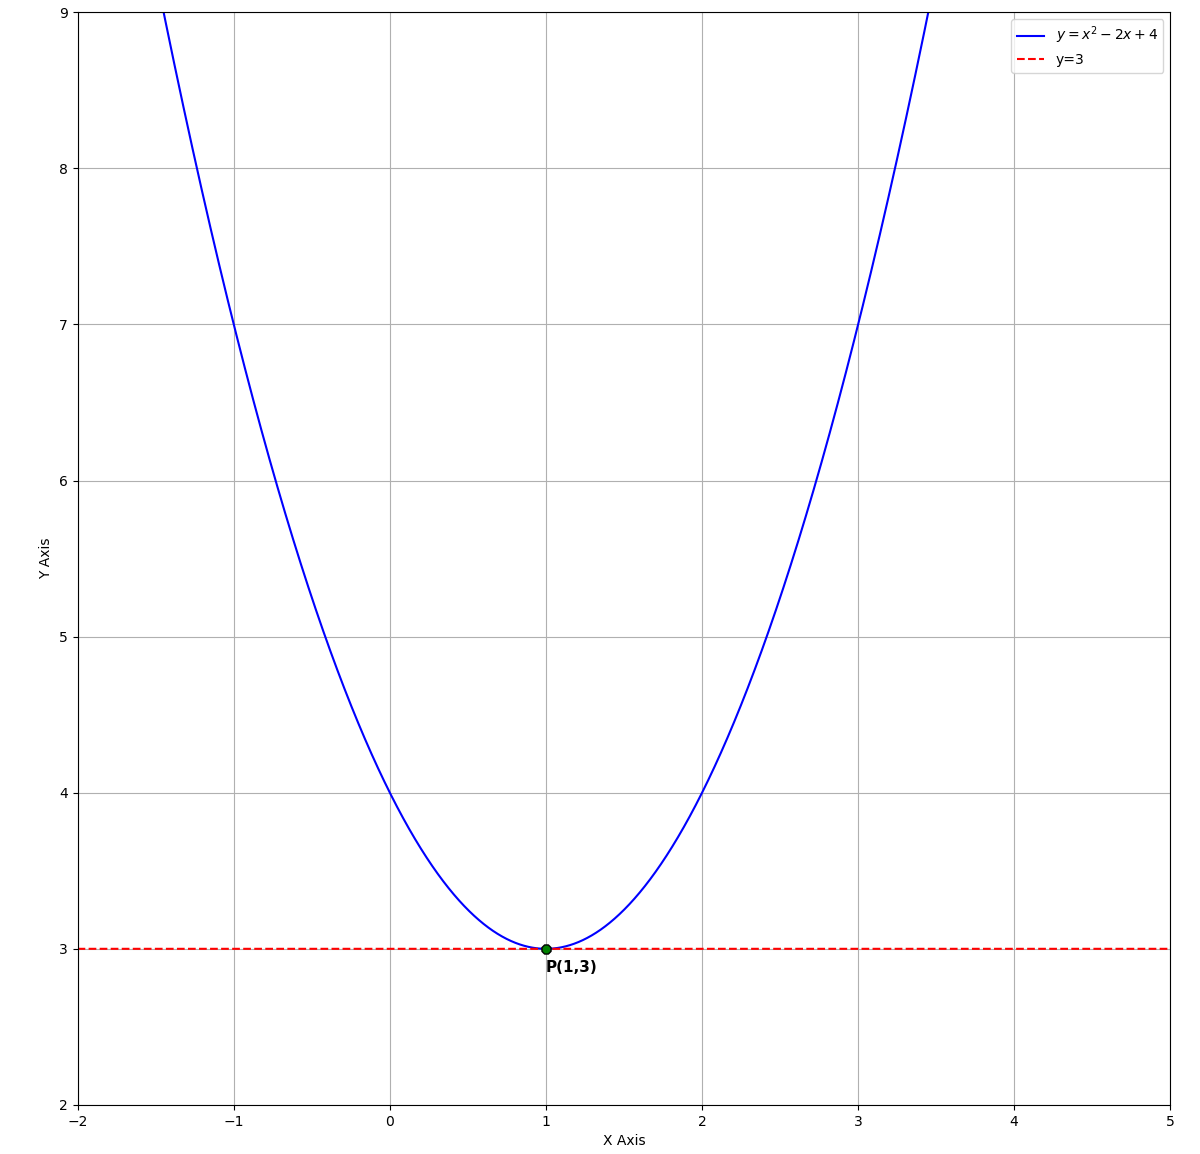
\includegraphics[width=\columnwidth]{figs/fig1.png}
    \caption{Parabola and Line}
    \label{fig:figs/fig1.png}
\end{figure}


\end{document}  
